\documentclass{article}
\usepackage{float}
\usepackage{hyperref}
\usepackage{booktabs}
\usepackage{tabularx}
\usepackage{apacite}
\usepackage[margin=1in]{geometry}
\usepackage{natbib}
\usepackage{setspace,caption}
\usepackage{csquotes}
\usepackage{epigraph}
\usepackage{amsmath}
\usepackage{dcolumn}
\usepackage{rotating}
\bibliographystyle{apa} 

\doublespacing

\title{The (In)effectiveness of Campaign Spending: \\ Evidence from California}
\author{Sahil Chinoy}
\date{May 15, 2017}

\begin{document}

\maketitle{}

\begin{displayquote}
``Politics has got so expensive that it takes lots of money to even get beat with.'' \\ -- \textit{Will Rogers}
\end{displayquote}

\section{Introduction}

Many Americans believe that our political system has been tarnished by the influence of money. Recently, Donald Trump was swept into office on a wave of populist resentment of a political establishment seen as irrevocably corrupt, in part because it continues to concentrate wealth amongst its members and other ``elites.'' On both sides of the political aisle, big donors -- individuals such as George Soros, corporations including oil and pharmaceutical companies, interest groups such as the NRA -- are generally resented, and in the wake of \textit{Citizens United v. FEC}, this problem seems to have grown more acute. According to the media, money continues to pour into political campaigns at an alarming and ever-increasing rate, and ``dark money'' devices seemingly allow candidates and their backers to keep more of their finances secret.

Yet, the effects of campaign spending are far from clear. For such a basic and important question -- how much does spending influence a candidate's chance of being elected, and which types of expenditure matter the most -- the economics and political science literatures are remarkably unresolved, and the only consensus seems to be that the effects are negligible or ambiguous, especially for incumbents. This raises the question of why candidates devote so much time and energy to raising money, if it's unclear that it will help them win. Moreover, it counters the narrative that money is increasingly corrupting our political system. If it is true that spending doesn't matter -- or doesn't matter much -- then the heated debates over campaign finance reform, spending caps, and public financing of campaigns can be resolved.

However, both the academic literature and much of the media coverage have focused on races for federal office, mainly the Senate and the House of Representatives. Candidates for local and state elections raise and spend money too, sometimes in surprisingly vast quantities. One might imagine that although the effects of spending at the federal levels are small or ambiguous, the smaller scale of elections for state office makes campaign spending more effective. As motivation, consider Figure \ref{fig:vote-share-spending}, which shows a clear relationship between spending and vote share in California state legislative races. Except when candidates dramatically outspend their opponents, it would appear as though campaign expenditure is effective.

\begin{figure}
  \centering
  \caption{Democratic vote share versus the amount by which Democratic candidates outspent Republicans. There is a positive relationship between spending and vote share. Data is for California Assembly races from 2002 to 2016.}
	\label{fig:vote-share-spending}
  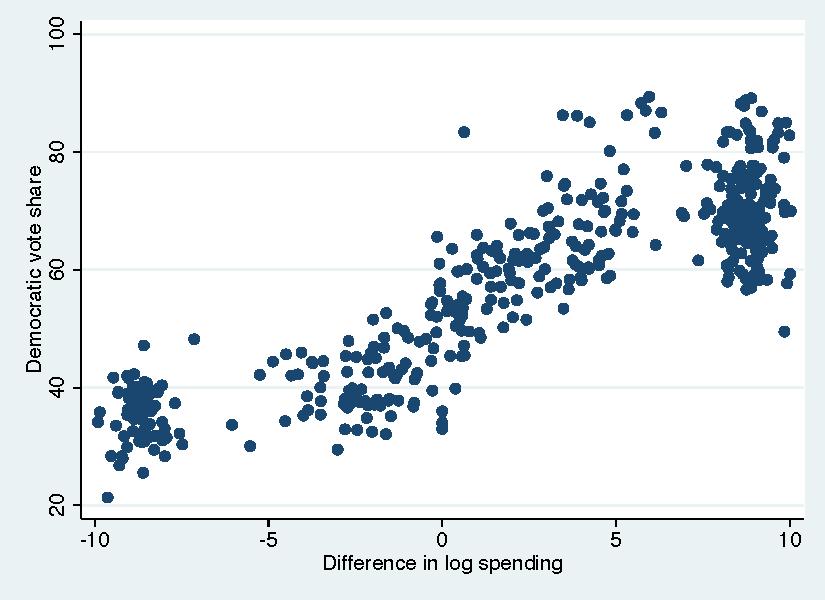
\includegraphics[width=.8\linewidth]{../charts/diff.pdf}
\end{figure}

This paper pursues the fundamental question in campaign finance: how many votes does an extra dollar of spending buy? It does so in the novel context of elections to the California Assembly. Using a new dataset of itemized expenditures, I conduct a detailed analysis of the relative effectiveness of \textit{types} of spending -- ads versus fundraisers, for example -- and estimate the degree to which spending on non-campaign activities such as administrative costs biases measurements of spending effectiveness. To account for endogeneity due to unobserved candidate quality, I focus on candidates who have run for office more than once.

The results, however, corroborate findings at the federal level: campaign spending in California Assembly races, regardless of category and accounting for measurement error, is remarkably ineffective. This means that the puzzle of why candidates continue to spend money on campaigning remains. The sole exception is advertising and communications spending for challengers, which lends support to theoretical models of campaign finance that see campaign spending as directly informative.

The rest of the paper proceeds as follows: Section Two reviews the relevant literature, Section Three summarizes the data on spending in California Assembly races, Section Four develops a model of campaign spending and discusses empirical strategy, Section Five presents the results, and Section Six concludes.

\section{Literature review}

\subsection{Theoretical models of campaign finance}

Why do candidates for political office raise and spend money? \cite{coleman2000congressional} argue that they spend ``to increase name recognition and public awareness of their views,'' but the exact mechanism by which this occurs is an open question. Models of campaign fundraising and spending usually involve some combination of candidates, political parties, interest groups, and voters. They assume that only political parties and special interests contribute to campaigns with the intention of winning political favors, and that spending is directed solely at winning votes.\footnote{ This assumption has been challenged by \cite{ansolabehere2003there}, who argue that individual donors are actually the major source of money in U.S. campaigns. In the wake of \textit{Citizens United v. Federal Election Commission (2010)}, this point is less salient.}$^,$\footnote{ Not necessarily in the current election. \cite{goodliffe2001effect} examines the intertemporal spending decisions of candidates with a ``war chest'' that persists across elections. \cite{milyo2001candidates} motivates this by modeling candidates as intertemporal utility maximizers.} Refining these models is important because different assumptions about the behavior of voters, contributors, and candidates lead to models with differing implications for campaign finance policy, including spending caps and public financing. 

In almost all of this literature, campaign spending is assumed to be exclusively on advertisement, a treatment that follows from earlier models in political economy outside the context of voting, for example \cite{kihlstrom1984advertising}. Some authors recognize that spending also includes canvassing and organizational costs such as campaign consultants and surveys, but because expenditures have historically been directed towards TV advertising, most models discount these other channels, according to \cite{prat2004rational}.

Obviously, any model needs to incorporate the fact that the more a candidate spends, the larger their vote share, all else equal. But the microfoundations of the mechanism by which advertising influences election outcomes is a topic of active investigation. There are two approaches to modeling the effects of advertising. The first assumes candidates use advertising to truthfully inform candidates about their positions and qualifications. This is the approach taken by \cite{coate2004pareto}, who finds that even under these ``optimistic assumptions'' (and the even more optimistic assumption that voters listen and update their beliefs), the fact that interest groups can contribute to campaigns in exchange for policy favors means that contribution limits might still be beneficial.\footnote{ Models with non-rational voters, perhaps with cognitive biases, are discussed in \cite{prat2004rational}.} \cite{ashworth2006campaign} also investigates the trade-off between directly informative advertising and the political favors necessary in order to finance them, predicting ambiguous effects of public financing.

The second approach, taken by \cite{prat2002campaign}, assumes that advertisements are not directly informative of a candidate's position or quality. Instead, the amount of money a candidate \textit{raises} (and thus spends) from interest groups signals to voters qualities that they, as individuals without access to the candidate, cannot observe directly.\footnote{ Most models make the assumption that a candidate spends all the money they raise.} In this framework, the act of spending money takes symbolic value: \cite{prat2004rational} argues that a high-quality candidate, confident that voters will elect them more than once, is more willing to spend money on advertisement than a candidate less certain about their re-election chances.\footnote{ This is suggestive of the endogeneity problem in \textit{estimating} these effects that will be discussed later.} Following a signaling model adapted from an earlier literature in political economy, namely \cite{milgrom1986price}, the model developed in \cite{potters1997campaign} suggests that campaign spending is effective as a signaling device only when voters' interests align with the candidate's, offering one theoretical motivation for varying estimates of the returns to campaign spending. 

Both of these modeling approaches lead to a similar conclusion: campaign spending enables voters to accurately learn about candidate quality, at the expense of politicians awarding favors to lobbying groups who contribute to their campaigns. However, if advertising is directly informative, then there may be a benefit to publicly financing campaigns; if its effects are indirect, then giving money to all candidates does not signal to voters any additional information about candidate quality.

Most models do not incorporate other types of expenditure -- on campaign consultants or overhead costs such as travel, for example. This is significant, because in the Californian context of this paper, candidates spend at least as much on these other forms of expenditure as on advertisements. By estimating the relative effectiveness of these forms of campaign spending, then, I aim to motivate the development of  theoretical models including these channels. If spending on campaign consultants is effective in driving votes, for example, then perhaps theoretical models should incorporate the candidate's decision to hire a consultant. As \cite{coate2004pareto} says, these are issues on which the existing empirical literature ``offers no guidance.''

\subsection{Empirical estimates of spending effectiveness}

How many votes does an extra dollar of campaign spending buy? Empirical study of this question faces a classic issue of endogeneity: high-quality candidates, or those who are more likely to win election regardless of spending, are also able to raise and spend more money. As a result, conflicting estimates of the effectiveness of campaign spending abound. According to \cite{milyo-1999}, ``no strong consensus has been reached on the importance of money in elections.'' 

There is one thread in this literature, beginning with \cite{jacobson-1978}, that uses proxies such as the incumbent's vote share in previous elections to control for omitted variables including candidate quality and district partisanship, then estimates the effectiveness of spending using OLS. But while Jacobson finds no significant effect of incumbent spending in the U.S. House, by changing the specification of his model and employing an eight-point scale to measure challenger quality, \cite{green1988salvation} find that incumbent spending has a substantial impact on vote share.\footnote{ Their paper begins a long and contentious back-and-forth about the effectiveness of incumbent spending in the House.} \cite{erikson1998campaign}, using a simultaneous equations approach, corroborate these results. \cite{gerber1998estimating} instruments using candidate wealth levels for U.S. Senate elections, finding higher returns to incumbent spending than previously estimated, implying that spending is a significant factor in creating the incumbency advantage in the Senate. Evidently, even approaches using proxy variables or TSLS can lead to significantly different results, depending on the measures of candidate quality and district-specific effects that are included. In general, however, the literature has historically found much greater returns to spending by challengers than by incumbents; \cite{moon-2006} attributes this to the fact that many incumbent seats are safe, and as \cite{stratmann2005some} argues, policy intended to mitigate the incumbency advantage in elections needs to understand these differential returns.

A seminal study with a novel approach is \cite{levitt-1994}, who uses repeat challengers in the U.S. House to control for candidate quality and district fixed effects. Levitt restricts his sample to only races in which the same two candidates face each other across multiple elections, and estimates returns to campaign spending about an order of magnitude smaller than previous studies, suggesting that proxy variables and constructed measures of candidate quality do not fully capture these latent attributes. I follow this identification strategy, first-differencing expenditures for repeat candidates in California Assembly elections in order to estimate the returns to different forms of campaign expenditure.

Since Levitt's work, the debate about the effectiveness of spending in federal congressional races seems to have slowed. Many researchers regard his research design as the most convincing to date. But as \cite{milyo2015money} emphasizes, the existing literature largely focuses on federal elections; little attention has been paid to the role of money in politics at the local and state level. In fact, the only study of returns to spending in state congressional races is \cite{stratmann2006contribution}, who shows that seemingly low estimates of the effectiveness of incumbent spending are due to the fact that incumbents are relatively uninhibited in spending, and thus because of diminishing returns to expenditure, varying their expenditure does not significantly alter their vote share. 

There is no good reason to believe the effectiveness of campaign spending is the same for federal and state elections. In fact, according to \cite{milyo2015money}, ``contributions to state and local office holders may be more influential than otherwise suggested by existing studies of contributions to federal legislators.'' I contribute to this literature not by asking a novel question or proposing a new identification strategy, but by asking the same question -- how many votes does a dollar of campaign expenditure buy -- in the novel context of state elections. If the models that suggest campaign spending informs voters about a candidate's quality and positions are correct, I expect campaign spending to be at least as effective at the state level, given that voters are less likely to be familiar with candidates or informed about their policy stances. I also investigate the magnitude of the incumbency advantage at the state level. If it is true that campaign spending is more effective in races for state office, I expect the incumbency advantage to be greater there as well.

Most studies of campaign finance use the total expenditure reported by candidates and their committees: the ``top-line'' numbers. However, total spending includes administrative costs such as phone bills and travel that might not directly influence election outcomes through the channels that the theoretical models, especially the truthful reporting model of \cite{coate2004pareto}, suggest. If all candidates spend an equal share of their funds on these expenses, then the effect should be negligible, but if some candidates spend a greater fraction of their total expenditure on, say, advertisement, then their returns to spending might be greater. \cite{ansolabehere1994mismeasure} address this measurement error by using itemized expenditure data for U.S. House races. They separate expenditure into three categories: spending that involves direct communication with voters, campaign-related spending that doesn't involve communication with voters (such as polling), and spending unrelated to campaigning (such as administrative costs). They find that subtracting non-campaign costs from total spending yields larger estimates of the effectiveness of spending; however, spending by incumbents is still insignificant (and actually has the wrong sign). I follow their methodology in attempting to separate the effects of campaign-related spending and overhead costs.

Studies that attempt to disentangle the various types of campaign spending, as opposed to analyzing the effects of spending writ large, have generally focused on TV ads. \cite{goldstein2000new} construct a measure of advertising exposure, find that it has significant effects on vote share, and argue that since money buys advertisements, money therefore influences elections. But they estimate an indirect effect of campaign spending -- it is not clear that a dollar spent by two candidates will increase each candidate's advertising exposure equally.\footnote{The significance of advertising in determining election outcomes is well-documented in the political science literature. See, for example, \cite{shaw1999effect}. The question I will attempt to answer is not about the influence of ads, but about the relative impact of campaign spending on advertisement \textit{vis-\`{a}-vis} other categories.} \cite{stratmann2009prices} estimates directly the effects of TV ad spending, taking into account the varying price of television airtime across regions. He finds statistically significant effects of spending on TV ads for both incumbents and challengers. Stratmann's paper is closest to this study -- he also employs Levitt's repeat challengers strategy -- however, he explores the effectiveness of one particular channel of expenditure rather than the candidate's decision to allocate campaign funds between advertisements, campaign consultants, fundraisers, etc.

Finally, previous studies of campaign expenditure other than advertisement have mostly been limited to field experiments. For example, \cite{adams1980effects} study the effects of telephone canvassing in a 1979 special election in Washington, D.C., finding limited impact on vote share. These studies, however, make no attempt to estimate the effectiveness of spending on these forms of campaigning in relation to TV or radio ads. Others, such as \cite{gerber2000effects}, focus exclusively on the effects of canvassing on voter turnout. Moreover, while there is a political science literature on the rise of campaign consultants in U.S. elections, no existing studies analyze empirically the effects of spending on information-gathering, including consultants and surveys. I estimate the relative effectiveness of this channel compared to advertisements and fundraisers.

\section{Data on itemized expenditures for California Assembly races}

I assemble a panel dataset from two sources. The first, the California Civic Data Coalition's refined version of the Secretary of State's CAL-ACCESS database, contains itemized expenditures for each candidate who has run for state office since 2000.\footnote{\url{http://www.californiacivicdata.org}}$^,$\footnote{Specifically, I identify all committees associated with a particular candidate, then aggregate each line-item expenditure reported by those committees on disclosure form F460 for the election cycle in question. For example, for the 2012 general election, I use expenditures from January 1, 2011 to December 31, 2012.} The expenditures are coded by category: for example, \texttt{CNS} denotes spending on campaign consultants. However, these categories are quite specific, and some filings code expenditures differently. So, following the treatment in \cite{ansolabehere1994mismeasure}, I aggregate the spending codes into five coarser categories, presented in Table \ref{table:categories}. I also use money spent on fundraisers as a separate category. The six categories for which I estimate relative effectiveness are then (1) direct communication with constituents; (2) print, TV, and radio ads; (3) information-gathering such as campaign consultants and polling; (4) contributions to other committees and donations; (5) overhead costs such as accounting services and salaries; and (6) fundraisers.

\begin{table}
\centering
\caption{Aggregation of expenditure codes into five coarse categories.}
\label{table:categories}
\begin{tabular}{l l l}
\toprule
\textbf{Communication} & \textbf{Ads} & \textbf{Information} \\ \midrule
campaign literature and mailings & print ads & campaign consultants \\
member communications & radio airtime and production costs & polling and survey research \\
phone banks & TV airtime and production costs & \\ \midrule
\textbf{Contributions} & \multicolumn{2}{l} { \textbf{Overhead} } \\ \midrule
contributions & \multicolumn{2}{l} {candidate filing/ballot fees} \\
civic donations & \multicolumn{2}{l} {legal defense} \\
& \multicolumn{2}{l} {meetings and appearances} \\
& \multicolumn{2}{l} {office expenses} \\
& \multicolumn{2}{l} {postage, delivery, and messenger services} \\
& \multicolumn{2}{l} {professional services (legal, accounting)} \\
& \multicolumn{2}{l} {campaign workers' salaries} \\
& \multicolumn{2}{l} {candidate travel, lodging, and meals} \\
& \multicolumn{2}{l} {staff/spouse travel, lodging, and meals} \\
& \multicolumn{2}{l} {information technology costs (internet, e-mail)} \\
\bottomrule
\end{tabular}
\end{table}

To the expenditure data, I add information on each candidate's vote share from the OpenElections project.\footnote{\url{https://github.com/openelections}} Data is available for the eight general elections from 2002 to 2016. Keeping only contested elections in which the candidate reported spending money, this results in expenditure information for 832 candidates. Summary statistics are presented in Table \ref{table:summary}.

\begin{table}
\begin{center}
\caption{Summary statistics for spending variables, vote share, and win percentage.}
\label{table:summary}
\newcolumntype{Y}{>{\raggedleft\arraybackslash}X}
\begin{tabularx} {\textwidth} {@{} l r Y Y Y Y Y Y Y Y Y Y Y Y Y Y Y@{}} \\
\toprule
\multicolumn{10}{c}{ } \\
& & \multicolumn{9}{c}{Mean} \\
\multicolumn{10}{c}{ } \\
&$N$&Total&Comm.&Ads&Info.&Fund.&Over.&Contrib.&Votes&Winner \\
\midrule
Challenger&545&\$66.5&\$13.9&\$12.3&\$9.6&\$2.2&\$15.4&\$4.4&51\%&52\% \\
Incumbent&287&\$88.6&\$7.6&\$11.7&\$9.6&\$5.9&\$17.1&\$17.8&65\%&97\% \\
\midrule
Democrat&468&\$85.1&\$11.0&\$12.9&\$11.4&\$4.2&\$19.4&\$12.2&61\%&76\% \\
Republican&364&\$60.1&\$12.6&\$11.1&\$7.2&\$2.5&\$11.7&\$5.0&50\%&56\% \\
\midrule
\textbf{Total}&832&\$74.1&\$11.7&\$12.1&\$9.6&\$3.5&\$16.0&\$9.0&56\%&67\% \\
\bottomrule
\multicolumn{10}{c}{ } \\
& & \multicolumn{9}{c}{Standard deviation} \\
\multicolumn{10}{c}{ } \\
\midrule
Challenger&545&\$828.9&\$206.4&\$391.4&\$111.3&\$33.7&\$190.1&\$74.1&15\%&50\% \\
Incumbent &287&\$747.1&\$123.1&\$382.6&\$89.9&\$57.1&\$184.6&\$150.6&9\%&17\% \\
\midrule
Democrat&468&\$759.7&\$134.8&\$393.3&\$108.9&\$52.9&\$195.6&\$134.6&14\%&43\% \\
Republican&364&\$846.8&\$233.2&\$381.8&\$93.3&\$35.2&\$169.0&\$95.6&14\%&50\% \\
\midrule
\textbf{Total}&832&\$808.1&\$184.5&\$388.2&\$104.4&\$46.8&\$188.3&\$124.3&15\%&47\% \\
\multicolumn{10}{c}{} \\
\bottomrule
\multicolumn{10}{l}{\footnotesize Spending variables in tens of thousands of dollars.}\\
\end{tabularx}
\end{center}
\end{table}


First, the magnitude of the incumbency advantage is stunning. Fully 97\% of the incumbents in this sample won re-election. They also outspent their opponents by more than \$200,000, on average. Interestingly, however, most of this extra spending was on fundraisers, overhead costs, and especially contributions to other candidates and committees. Challengers outspent incumbents on direct communication with voters and on TV, print, and radio advertisements. This makes sense -- challengers need to make their presence known, and thus spend more money on communication with voters than incumbents, who are more likely to be known by their constituencies.

There are more Democrats than Republicans in this sample, and Democrats are far more likely to win election. This reflects the political climate of California. It is interesting, however, that Republicans spend more on communication with voters than Democrats.

Finally, for all candidates, the largest spending category by far is overhead costs: office expenses, salaries, and travel. These administrative costs are unlikely to have a direct impact on vote share: if a candidate can run the same campaign with smaller phone bills, for example, then their ultimate vote share should not be impacted.\footnote{Unless, of course, their ability to save money is correlated with their intrinsic electability, which is not implausible.} This motivates an estimate of the effectiveness of non-overhead, non-contribution campaign spending including communication, ads, information, and fundraisers. I construct this category, which I call ``general'' spending, following \cite{ansolabehere1994mismeasure}.

\begin{table}
\centering \caption{Cross-correlations of spending variables in logarithmic form. \label{table:corr}}
\begin{tabular}{l c  c  c  c  c  c  }\toprule
\multicolumn{1}{c}{} &Total&Comm.&Ads&Info.&Fund.&Overhead\\ \midrule
Comm.&0.71\\
Ads&0.50&0.44\\
Info.&0.79&0.65&0.36\\
Fund.&0.75&0.47&0.29&0.61\\
Overhead&0.86&0.72&0.46&0.76&0.69\\
Contrib.&0.63&0.25&0.03&0.5&0.69&0.51\\
\bottomrule

 \end{tabular}
\end{table}

Table \ref{table:corr} presents cross-correlations between the spending variables, entered in logarithmic form.\footnote{This is standard in much of the economics literature but not always in political science -- compare, for example, \cite{ansolabehere1994mismeasure} to \cite{jacobson-1978}. I found the correlations to be more robust with logarithmic spending.} Among the spending categories (which are mutually exclusive), the strongest correlations are between overhead costs and information and between overhead and communications. This is likely due to the fact that candidates running a bigger campaign with more overhead costs also spend more on other categories. In general, however, the correlations between spending variables are not particularly large, which motivates a regression designed to estimate the effectiveness of spending more money on each category, holding other channels constant.

The correlation between advertisements and all other categories is particularly weak. Figure \ref{fig:ads} displays the relationship between total spending and spending on ads, and shows that there are many candidates with low ad spending given their total spending.\footnote{This finding is robust to separating candidates by incumbency status.} This suggests that some candidates might consciously \textit{decide} to spend more on ads -- larger ad spending does not simply indicate a larger campaign -- which would lend support to theoretical models that focus on a candidate's decision to spend money exclusively on advertisements.

\begin{figure}
  \centering
  \caption{Ad spending versus total spending. Some candidates spend a disproportionately small amount on advertisement relative to their total expenditure.}
  \label{fig:ads}
  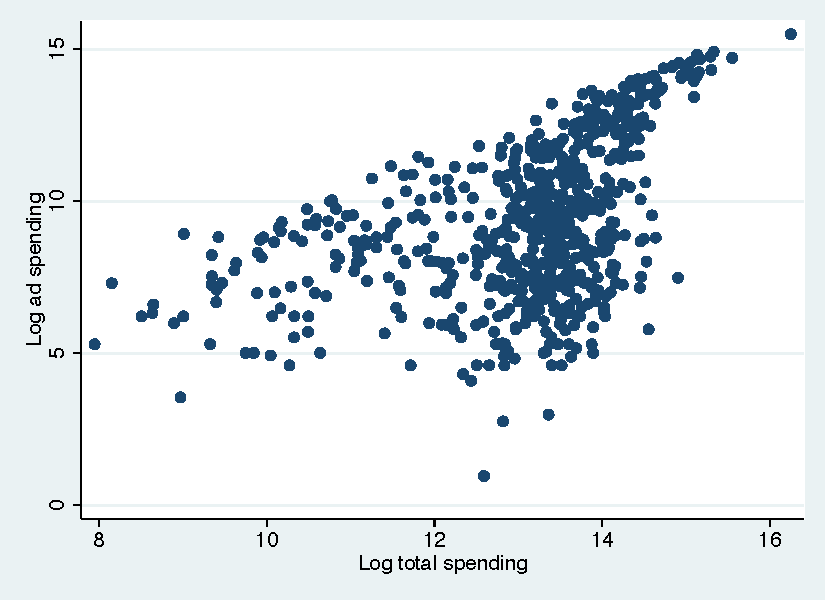
\includegraphics[width=.8\linewidth]{../charts/ads.pdf}
\end{figure}

\section{Model and empirical strategy}

My model of election outcomes follows directly from \cite{levitt-1994}. I extend his work, however, by estimating the model using expenditure on specific categories in order to gauge the relative effectiveness of different types of spending.

\subsection{A simple model of campaign spending}

Although the unit of observation in the data is an individual candidate, I model spending at the race level, rather than the candidate level, since the spending of a candidate's opponent is relevant to the candidate's own spending decisions. To simplify, I restrict attention to only elections in which one Democrat faces off against one Republican and both candidates have nonzero spending.\footnote{This is a significant restriction in the context of this sample. Further work could extend this model to races in which a candidate runs unopposed, or two candidates from the same party vie for the same seat. This is particularly relevant in primary elections and has not been extensively studied.}

Let $V_{it}$ be the Democratic vote share in district $i$ in election $t$. Let $I_{it}$ be an indicator that equals one if the Democratic candidate is the incumbent in district $i$ in election $t$, negative one if the Republican candidate is the incumbent, and zero otherwise.\footnote{This model appears at first more cumbersome than simply using the incumbent vote share as the dependent variable. Importantly, however, it allows us to enter races for an open seat (no incumbent) in the same model. This is especially important for the state races in this sample.} Let $\text{INC}_{it}$ be the expenditure by the incumbent, $\text{CHAL}_{it}$ be the expenditure by the challenger, and $\text{OPEN}_{it}$ be the difference in total spending between Democrats and Republicans for an open-seat election.\footnote{One in which there is no incumbent.} I enter all spending variables in logarithmic form.\footnote{I estimated the models using linear expenditure, but found the logarithmic form better explained the variation in vote share. This makes sense, given that campaign expenditure likely has diminishing returns to scale. To win extra votes, one must outspend their opponent by orders of magnitude.}

Now, assume vote share is also driven by an (unobserved) measure of each candidate's valence or quality $\text{VAL}_{i}$, which is constant for each candidate. Let $\text{VAL}^D_{it}$ be the valence of the Democratic candidate and $\text{VAL}^R_{it}$ be the valence of the Republican candidate. Note that these terms are indexed by the election $t$ because the identity of the candidate in each district can change between elections. I also account for the partisan alignment of a district using the \textit{average} Democratic share of the congressional vote over the elections in our sample, $\text{DIST}_{i}$. By construction, this does not change over time.\footnote{Contrast with models incorporating the lagged Democratic vote share.} Finally, I account for election fixed effects such as nationwide partisan shocks with $\gamma_t$. In the 2010 midterm elections, for example, all Democrats fared worse, and I want to disentangle this effect from campaign spending. Assume the error term $\epsilon_{it}$ is independent and identically distributed. Then the model is

\begin{equation}
\text{V}_{it} = \alpha \, \text{DIST}_i + \delta_1 \, \text{VAL}^{D}_{it} + \delta_2 \, \text{VAL}^{R}_{it} + I_{it} \times (\eta + \beta_1 \, \text{INC}_{it} + \beta_2 \, \text{CHAL}_{it}) + \beta_3 \, \text{OPEN}_{it} + \gamma_t + \epsilon_{it}.
\label{eq:full}
\end{equation}

I expect $\alpha$ and $\delta_1$ to be positive and $\delta_2$ to be negative. The coefficients on incumbent and open-seat spending, $\beta_1$ and $\beta_3$, are expected to be positive, and $\beta_2$ should be negative. Here, $\eta$ captures the non-spending benefits of incumbency; I expect it to be positive as well.

The fundamental problem is that no measure of candidate valence exists in the data.\footnote{One could try to construct a measure of valence, but \cite{levitt-1994} shows that these measures likely do not capture the full effect.} This means that an estimate of Eq. (\ref{eq:full}) will suffer from omitted variable bias. In particular, since I expect a positive correlation between candidate valence and candidate spending and between candidate valence and vote share, the spending coefficients $\beta$ will likely be inflated in magnitude.

Still, following \cite{jacobson-1978}, estimating Eq. (\ref{eq:full}) without including candidate valence is useful for the following reasons. First, assuming that the relationship between valence and spending is roughly the same for incumbents, challengers, and candidates for open seats, it is still possible to gauge the relative effectiveness of expenditure for these types of candidates. Second, assuming the relationship between valence and each \textit{form} of spending is roughly the same, it is possible to gauge the relative effectiveness of total spending and general spending to identify the effects of measurement error, following \cite{ansolabehere1994mismeasure}. These are, of course, nontrivial assumptions: our estimates, though biased, must be \textit{consistently} biased.

\subsection{Identification via first-differencing}

An alternative strategy is to restrict the sample to \textit{repeat} candidates: candidates that run for the same office in the same district twice. Note that while this is in the same spirit as Levitt's repeat challengers approach, I allow the identity of the opposing candidate to change between elections. This compromise ensures the sample size is sufficiently large. First-differencing Eq. (\ref{eq:full}) thus eliminates \textit{one} candidate valence term and the district partisan alignment term, and results in

\begin{equation}
\Delta \text{V}_{i} = \delta \, (\Delta \text{VAL}_i) + \eta \, (\Delta I_{i}) + \beta_1 \, \Delta (I_i \times \text{INC}_{i}) + \beta_2 \, \Delta (I_i \times \text{CHAL}_{i}) + \beta_3 \, (\Delta \text{OPEN}_{i}) + \Delta \gamma + \epsilon_{i}
\label{eq:diff1}
\end{equation}

where the index $i$ runs over all candidates $j$ who appear in a \textit{pair} of elections $(t_1, t_2)$. The symbol $\Delta$ indicates the difference in the variable between elections $t_1$ and $t_2$. The district partisan alignment term and one valence term drop out, but another valence term, $\Delta \text{VAL}$, for which there is no measure, still appears in the equation. However, assuming that the quality of a particular party's candidate in a district does not change dramatically from year to year, then this term will be small. This specification will almost certainly suffer from a smaller omitted variable bias than specification (\ref{eq:full}).

Ideally, however, I would restrict the sample to just repeated \textit{pairs} of candidates; candidates who face off against each other in the same district more than once. If the identity of neither candidate changes between elections, then first-differencing Eq. (\ref{eq:full}) results in

\begin{equation}
\Delta \text{V}_{i} = \eta \, (\Delta I_{i}) + \beta_1 \, \Delta (I_i \times \text{INC}_{i}) + \beta_2 \, \Delta (I_i \times \text{CHAL}_{i}) + \beta_3 \, (\Delta \text{OPEN}_{i}) + \Delta \gamma + \epsilon_{i}
\label{eq:diff2}
\end{equation}

where the index $i$ runs over all \textit{pairs} of candidates $(j, k)$ who appear in a pair of elections $(t_1, t_2)$. This specification is theoretically free of any omitted variable bias, but is difficult to estimate reliably because there are only 34 instances in which the same two candidates face off against each other and report nonzero spending.

I estimate both Eq. (\ref{eq:diff1}) and Eq. (\ref{eq:diff2}) for total and general expenditure. Note that I estimate these models without a constant term; if there are no spending changes, no changes in candidate incumbency or valence and no nationwide shock, then the change in Democratic vote share should be zero.

\subsection{Incorporating expenditure categories}

Instead of using total or general expenditure, by adapting the model slightly, I measure the relative effectiveness of the various categories of expenditure. I enter the six forms of expenditure in the data -- communications, ads, information, contributions, overhead, and fundraising -- explicitly. Let $k\in \{1,\ldots,6\}$ be an index that runs over these six spending variables for incumbents, $\text{INC}_{it}^k$, challengers, $\text{CHAL}_{it}^k$, and the difference in Democratic and Republican expenditure for open-seat elections, $\text{OPEN}_{it}^k$. Note that the spending categories are mutually exclusive. Then the model becomes

\begin{multline}
\text{V}_{it} = \alpha \, \text{DIST}_i + \delta_1 \, \text{VAL}^{D}_{it} + \delta_2 \, \text{VAL}^{R}_{it} \\ + I_{it} \times \bigg( \eta + \sum \limits_{k=1}^6 \beta^k_1 \, \text{INC}^k_{it} + \sum \limits_{k=1}^6 \beta^k_2 \, \text{CHAL}^k_{it} \bigg) + \sum \limits_{k=1}^6  \beta^k_3 \, \text{OPEN}^k_{it} + \gamma_t + \epsilon_{it}.
\label{eq:breakdown-full}
\end{multline}

First-differencing Eq. (\ref{eq:breakdown-full}) by candidate and by matchup as done previously yields the following models:

\begin{equation}
\Delta \text{V}_{i} = \delta \, (\Delta \text{VAL}_i) + \eta \, (\Delta I_{i}) + \sum \limits_{k=1}^6 \beta^k_1 \, \Delta ( I_i \times \text{INC}^k_{i} ) + \sum \limits_{k=1}^6 \beta^k_2 \, \Delta ( I_i \times \text{CHAL}^k_{i} ) + \sum \limits_{k=1}^6 \beta_3^k \, (\Delta \text{OPEN}^k_{i}) + \Delta \gamma + \epsilon_{i}
\label{eq:breakdown-diff1}
\end{equation}

where $i$ runs over repeat candidates, and

\begin{equation}
\Delta \text{V}_{i} = \eta \, (\Delta I_{i}) + \sum \limits_{k=1}^6 \beta^k_1 \, \Delta ( I_i \times \text{INC}^k_{i} ) + \sum \limits_{k=1}^6 \beta^k_2 \, \Delta ( I_i \times \text{CHAL}^k_{i} ) + \sum \limits_{k=1}^6 \beta_3^k \, (\Delta \text{OPEN}^k_{i}) + \Delta \gamma + \epsilon_{i}
\label{eq:breakdown-diff2}
\end{equation}

where $i$ runs over repeated matchups.

The coefficients $\beta_i^k$ capture the effects of a particular form of campaign expenditure, holding spending on other channels constant. For example, the coefficient $\beta_1^2$ captures the effect of spending on advertisements for incumbents, holding spending on communications, information, contributions, overhead, and fundraising fixed. I again expect $\beta_1^k$ and $\beta_3^k$ to be \textit{a priori} positive and $\beta_2^k$ to be negative for each spending category $k$.

\section{Results}

\subsection{Total spending}


\begin{table}
\centering
\def\sym#1{\ifmmode^{#1}\else\(^{#1}\)\fi}
\caption{Effectiveness of total versus general campaign spending. \label{table:reg}}
\begin{tabular}{l*{6}{c}}
\toprule
                    &\multicolumn{2}{c}{(1)}&\multicolumn{2}{c}{(2)}&\multicolumn{2}{c}{(3)}\\
                    &\multicolumn{1}{c}{Total}&\multicolumn{1}{c}{General}&\multicolumn{1}{c}{Total}&\multicolumn{1}{c}{General}&\multicolumn{1}{c}{Total}&\multicolumn{1}{c}{General}\\
\midrule
Incumbent spending  &        0.72         &        0.13         &        0.03         &        0.01         &        0.07         &       -0.28         \\
                    &      (0.95)         &      (0.35)         &      (0.61)         &      (0.26)         &      (2.06)         &      (1.29)         \\
\addlinespace
Challenger spending &       -1.09\sym{***}&       -1.24\sym{***}&       -0.67\sym{***}&       -0.67\sym{***}&       -0.30         &        0.06         \\
                    &      (0.21)         &      (0.23)         &      (0.14)         &      (0.14)         &      (0.41)         &      (0.53)         \\
\addlinespace
Open-seat spending  &        1.43\sym{***}&        1.53\sym{***}&        0.32\sym{**} &        0.28\sym{*}  &       -0.07         &       -0.45         \\
                    &      (0.10)         &      (0.12)         &      (0.12)         &      (0.13)         &      (0.32)         &      (0.31)         \\
\addlinespace
Incumbency          &        8.86         &       17.41\sym{***}&        7.35         &        6.92\sym{*}  &        1.47         &        1.48         \\
                    &     (11.79)         &      (3.44)         &      (7.95)         &      (3.11)         &     (27.23)         &     (13.20)         \\
\addlinespace
District alignment  &        0.30\sym{***}&        0.29\sym{***}&                     &                     &                     &                     \\
                    &      (0.04)         &      (0.04)         &                     &                     &                     &                     \\
\addlinespace
Constant            &       36.40\sym{***}&       36.59\sym{***}&                     &                     &                     &                     \\
                    &      (1.88)         &      (1.92)         &                     &                     &                     &                     \\
\midrule
Observations        &         459         &         459         &         282         &         282         &          34         &          34         \\
Adjusted \(R^{2}\)  &        0.84         &        0.84         &        0.11         &        0.11         &       -0.05         &       -0.01         \\
\bottomrule
\multicolumn{7}{l}{\footnotesize Robust standard errors in parentheses.}\\
\multicolumn{7}{l}{\footnotesize Dependent variable is Democratic vote share. Year fixed effects absorbed.}\\
\multicolumn{7}{l}{\footnotesize \sym{*} \(p<0.05\), \sym{**} \(p<0.01\), \sym{***} \(p<0.001\)}\\
\end{tabular}
\end{table}

The first two columns of Table \ref{table:reg} present the results of estimating specification (\ref{eq:full}) for the 459 races in the sample. Notice that campaign spending appears significant for challengers and contenders in open-seat elections, but not for incumbents. This is in line with most empirical campaign finance research, especially the simple model developed by \cite{jacobson-1978}. The problem seems to be that the magnitude of the incumbency advantage is so large that extra spending by incumbents is essentially pointless. This is especially true in the California sample -- recall that 97\% of candidates win re-election.

In contrast, spending appears significant for challengers, and even more so for open-seat contenders. The results of the first model imply that an approximately threefold increase in challenger spending is associated with a 1.1 percentage point increase in vote share, while a threefold increase in the difference in spending between two open-seat contenders is associated with a 1.4 percentage point increase in vote share.\footnote{Because the model is estimated using the natural logarithm of the spending variables, and $e \approx 3$.}

Consider the regression of total spending versus general spending -- which removes overhead costs, contributions to other committees, and uncategorized expenditures -- and note the slight increase in the effectiveness of spending for challengers and open-seat candidates, but not for incumbents, for whom the coefficient remains insignificant. This is in line with what I expect: spending on categories that directly reach voters or that increase a candidate's information about the race is expected to be more effective than spending on travel, for example. Like \cite{ansolabehere1994mismeasure}, then, I conclude that mismeasurement of spending is likely non-negligible, but does not explain the puzzle of ineffective incumbent spending at the state level.

The next two columns present the results of estimating specification (\ref{eq:diff1}) for the 282 repeat candidates in the sample. Recall that this specification removes some of the omitted variable bias due to an inability to measure candidate valence and an imperfect measure of district partisanship. Although the coefficients on challenger and open-seat spending are still significant, they are vastly reduced in magnitude. In particular, the effectiveness of challenger spending is reduced by a factor of two, and the effectiveness of open-seat spending is reduced by a factor of almost five. These results are in line with the substantive conclusions of \cite{levitt-1994}, who finds that the magnitude of the coefficient on challenger spending is far smaller in the first-differenced model, suggesting that the omitted variable bias in the un-differenced specification is significant. This is confirmed by noticing that $R^2$, the proportion of variation in vote share explained by the model, drops dramatically when we eliminate some candidate fixed effects in this way. The fact that the estimate drops more for open-seat contenders suggests that the correlation between candidate quality and spending or between quality and vote share is stronger for open-seat contenders than for challengers; i.e. latent characteristics determine the outcome to a greater degree when there is no incumbent.

After first-differencing, then, I conclude that campaign spending is largely ineffective -- it is mostly insignificant, except for challengers, for whom the effects are quite small. Note that using general spending as opposed to total expenditure does not change these results. These findings accord with most prior research that finds that incumbent spending is far less effective than challenger spending; the most common explanation in the literature is that incumbents are not restricted in funding and thus diminishing returns to scale make the effects of any change in expenditure negligible.\footnote{See \cite{stratmann2006contribution}, but note that this explanation is by no means universally accepted.}

Finally, the last two columns present the results of estimating specification (\ref{eq:diff2}) for pairs of repeat challengers, of which there are only 34 in this sample. Because of the small sample size, these estimates are very noisy. The point estimates shrink compared to the previous specifications, but because the standard errors grow significantly, it's difficult to discern whether this is simply noise, or the genuine effect of further removing omitted variable bias. I present them for completeness. 

\subsection{Relative impact by expenditure category}

\begin{table}
\centering
\def\sym#1{\ifmmode^{#1}\else\(^{#1}\)\fi}
\caption{Relative impact of campaign spending on vote share by expenditure category. \label{table:breakdown}}
\begin{tabular}{l*{3}{cc}}
\toprule
                    &\multicolumn{2}{c}{(4)}           &\multicolumn{2}{c}{(5)}           &\multicolumn{2}{c}{(6)}      \\
\midrule
Incumbent communications&       -0.97\sym{***}&      (0.26)&       -0.42         &      (0.24)&       -0.96         &      (1.70)\\
Incumbent ads       &        0.38\sym{**} &      (0.14)&        0.05         &      (0.15)&       -1.09         &      (0.62)\\
Incumbent information&        0.27         &      (0.24)&        0.15         &      (0.21)&        0.26         &      (1.13)\\
Incumbent fundraising&        0.84\sym{*}  &      (0.41)&        0.32         &      (0.40)&        1.57         &      (1.52)\\
Incumbent overhead  &       -0.41         &      (0.50)&        0.39         &      (0.46)&        2.93         &      (3.71)\\
Incumbent contributions&        1.54\sym{***}&      (0.43)&        0.60         &      (0.45)&       -1.20         &      (3.18)\\ \midrule
Challenger communications&       -0.92\sym{**} &      (0.34)&       -0.59\sym{*}  &      (0.28)&       -1.72         &      (1.71)\\
Challenger ads      &       -0.66\sym{*}  &      (0.28)&       -0.64\sym{**} &      (0.24)&       -0.77         &      (0.97)\\
Challenger information&       -0.51         &      (0.42)&        0.11         &      (0.27)&        1.77         &      (0.98)\\
Challenger fundraising&        0.33         &      (0.57)&        0.37         &      (0.31)&        0.19         &      (0.94)\\
Challenger overhead &        0.71\sym{*}  &      (0.34)&        0.08         &      (0.27)&        0.20         &      (1.15)\\
Challenger contributions&       -0.59         &      (0.43)&        0.21         &      (0.23)&        0.06         &      (0.49)\\ \midrule
Open-seat communications&        0.02         &      (0.23)&        0.28         &      (0.22)&       -0.09         &      (1.19)\\
Open-seat ads       &       -0.23         &      (0.16)&       -0.03         &      (0.12)&       -0.55         &      (0.41)\\
Open-seat information&        0.04         &      (0.29)&       -0.20         &      (0.24)&       -1.67         &      (1.13)\\
Open-seat fundraising&        0.76\sym{**} &      (0.23)&        0.37         &      (0.24)&        0.87         &      (1.18)\\
Open-seat overhead  &        0.46         &      (0.30)&       -0.16         &      (0.29)&        0.73         &      (1.41)\\
Open-seat contributions&        0.88\sym{***}&      (0.23)&        0.38         &      (0.22)&        0.82         &      (1.69)\\ \midrule Incumbency          &        2.21         &      (6.71)&       -5.47         &      (6.02)&      -15.39         &     (33.20)\\
District alignment  &        0.25\sym{***}&      (0.03)&                     &            &                     &            \\
Constant            &       37.87\sym{***}&      (1.74)&                     &            &                     &            \\
\midrule
Observations        &         459         &            &         282         &            &          34         &            \\
Adjusted \(R^{2}\)  &        0.87         &            &        0.15         &            &       -0.13         &            \\
\bottomrule
\multicolumn{7}{l}{\footnotesize Robust standard errors in parentheses.}\\
\multicolumn{7}{l}{\footnotesize Dependent variable is Democratic vote share. Year fixed effects absorbed.}\\
\multicolumn{7}{l}{\footnotesize \sym{*} \(p<0.05\), \sym{**} \(p<0.01\), \sym{***} \(p<0.001\)}\\
\end{tabular}
\end{table}


Table \ref{table:breakdown} presents the results of estimating models (\ref{eq:breakdown-full}), (\ref{eq:breakdown-diff1}), and (\ref{eq:breakdown-diff2}), which incorporate expenditure categories.

Beginning with the first column (the un-differenced specification), there are only a few categories of expenditure that appear to significantly drive votes, but the coefficients do not always have the signs I expect. In particular, more spending on communication by incumbents seems to \textit{decrease} vote share. There is a long and confusing history of finding negative coefficients on incumbent spending in this literature -- see, for example, \cite{ansolabehere1994mismeasure}. The explanation is probably that the more a candidate needs to spend on communication, the less likely they are to be elected in the first place.\footnote{This too is omitted variable bias, but in the opposite direction from that which was described previously.} In contrast, contributing to other campaigns appears to be effective for incumbents. Again, this is probably due not to the fact that incumbent spending on contributions is especially effective, but due to the fact that incumbents who contribute to other campaigns are inherently more likely to be elected.

Examining the challenger coefficients, only communications and ads are moderately significant (with the right sign), and the point estimates are small. This accords with my intuition; for challengers, the most important use of campaign funds is likely to increase awareness and get one's name out. It also agrees with the literature that regards campaign spending as directly informative.

For open-seat contenders, fundraising and contributions are the most significant in driving votes. It is somewhat difficult to interpret the effects of spending on fundraisers -- this seems like spending money for the sake of raising more money to spend. If anything, this would support the theoretical models developed by, among others, \cite{prat2002campaign}, in which spending functions mainly as a signaling device: fundraising does not directly reach voters, but might contribute to the appearance of a well-funded, well-run campaign. However, these estimates are also likely to suffer significantly from omitted variable bias -- high-quality candidates are likely to have the easiest time raising funds, and well-connected candidates are likely to contribute to other campaigns. 

Even though these results are likely biased by an inability to control for candidate quality, the fact that each type of candidate has different spending categories associated with electoral success suggests that each type of candidate -- incumbents, challengers, and open-seat contenders -- makes spending decisions differently. This is an area ripe for future study. Note that spending on information gathering -- campaign consultants, surveys, and polling -- do not appear significant for any type of candidate, even in this un-differenced model. This is interesting, given that this category makes up a significant fraction of total expenditure, and is also largely unstudied.

However, upon first-differencing the model according to specification (\ref{eq:breakdown-diff1}), the only coefficients that remain large and significant are those on communications and advertising spending for challengers. Moreover, accounting for candidate quality in this way reduces the estimates of incumbent communications and contribution spending, and of open-seat fundraising and contribution spending. This is evidence that the estimates for fundraising and campaign contributions indeed suffer from significant omitted variable bias. The estimates are still noisy, and the effects of candidate quality are not fully eliminated, but this suggests that the most effective form of campaign expenditure is on advertisement and voter communications for challengers. Spending on other categories, and spending by other types of candidates, is largely ineffective. This provides empirical support for models of campaign finance such as those presented in \cite{coate2004pareto} that assume money spent by a candidate directly informs their constituents about their policies and characteristics, with the caveat that this is only true for challengers. It does not provide significant evidence for or against indirect signaling models such as those presented by \cite{prat2002campaign}, since in those models, the effects of spending are largely related to candidate quality, an effect which we have tried to remove via first-differencing.

Finally, using repeat challengers for specification (\ref{eq:breakdown-diff2}), I once again find that the sample size is not sufficiently large to precisely estimate the spending coefficients; in particular, the adjusted $R^2$ value suggests that this model is not well-estimated.

\subsection{Robustness}

One might imagine that the effectiveness of campaign spending would differ according to a number of characteristics about the race, district, and election cycle. An important characteristic is the competitiveness of a race -- it is reasonable that spending would be more effective in more competitive races. In this context, competitiveness can be defined in two ways: the closeness of the ultimate vote and the magnitude of the difference in campaign spending. In addition, it is conceivable that spending has grown more or less effective over time, due to changes in the institutional characteristics of elections in California.

Here, I check the results estimated from specification (\ref{eq:diff1}) using a subset of races. Table \ref{table:robustness} presents the results of four regressions: (1), using races for which the ultimate Democratic vote share was between 40 and 60 percent; (2), using races for which the difference in log spending between Democrats and Republicans was less than five; (3) using races during and after the 2010 general election; and (4), using races before the 2010 election. These results should be compared to the the estimates from specification (\ref{eq:diff1}) using general spending in Table \ref{table:reg}.

\begin{table}
\centering
\def\sym#1{\ifmmode^{#1}\else\(^{#1}\)\fi}
\caption{Robustness checks. \label{table:robustness}}
\begin{tabular}{l*{4}{c}}
\toprule
                    &\multicolumn{1}{c}{Competitive (votes)}&\multicolumn{1}{c}{Competitive (spending)}&\multicolumn{1}{c}{2010 and after}&\multicolumn{1}{c}{Before 2010}\\
\midrule
Incumbency          &        5.93         &        1.85         &        5.04         &        6.81         \\
                    &     (12.49)         &     (12.15)         &      (9.64)         &      (3.47)         \\
\addlinespace
Incumbent spending  &        0.22         &        1.44         &        0.20         &        0.05         \\
                    &      (1.07)         &      (1.35)         &      (0.86)         &      (0.30)         \\
\addlinespace
Challenger spending &       -0.79\sym{**} &       -1.77\sym{*}  &       -0.78\sym{**} &       -0.74\sym{*}  \\
                    &      (0.26)         &      (0.80)         &      (0.26)         &      (0.31)         \\
\addlinespace
Open-seat spending  &        0.50\sym{*}  &       -0.28         &        0.30         &        0.19         \\
                    &      (0.19)         &      (0.81)         &      (0.20)         &      (0.25)         \\
\midrule
Observations        &          52         &          51         &         125         &         100         \\
Adjusted \(R^{2}\)  &        0.23         &        0.03         &        0.12         &        0.12         \\
\bottomrule
\multicolumn{5}{l}{\footnotesize Robust standard errors in parentheses.}\\
\multicolumn{5}{l}{\footnotesize Spending variables are general spending. Dependent variable is Democratic vote share.}\\
\multicolumn{5}{l}{\footnotesize  Year fixed effects absorbed.}\\
\multicolumn{5}{l}{\footnotesize \sym{*} \(p<0.05\), \sym{**} \(p<0.01\), \sym{***} \(p<0.001\)}\\
\end{tabular}
\end{table}

Observe that the coefficients on challenger spending for competitive elections increase dramatically for competitive elections defined by spending, but the coefficients for incumbent and open-seat spending remain small and largely insignificant. This suggests that in competitive elections, spending by challengers might have a more significant impact than in uncompetitive elections in which the incumbent gains a significant advantage by vastly outspending the others. Importantly, however, the magnitude of the point estimates are still low -- it takes significantly more spending to produce a significant difference in vote share -- and are negligible for incumbents and for open-seat contenders. Spending, while more effective for challengers in competitive races, still cannot be considered an important driver of votes, especially given that the model fails to explain most of the variation in vote share.

Finally, upon estimating the model using elections prior to 2010 and after 2010 independently, there is essentially no difference between the coefficients. This suggests that campaign spending has not grown any more or less effective over time.

\section{Conclusion}

Addressing endogeneity in empirical study of campaign finance is an active area of research, and is critical in order to answer a fundamental question of vital importance: how effective is campaign spending? The literature has concluded that controlling for candidate quality through any sort of proxy is not quite good enough. In addition, separating the true effects of increased spending from the noise -- nationwide partisan shifts, idiosyncratic changes in spending, even shocks to the price of advertising -- is difficult, and thus there is no accepted conclusion about the effectiveness of campaign expenditure. These problems are exacerbated at the state level, where candidate quality can vary significantly, where the incumbency advantage is even stronger, and where district partisanship is often more dramatic. As a result of these issues and a lack of available data, existing work has almost exclusively focused on races for the U.S. Senate and House of Representatives.

In this paper, I extend existing approaches, models, and methodology to California State Assembly races from 2002 to 2016. I do so in the hopes of gauging whether campaign spending has a significantly different impact at the state level, and in particular whether the puzzle of ineffective incumbent spending remains. For methodological guidance, I draw primarily on two studies: \cite{ansolabehere1994mismeasure}, who address mismeasurement of campaign spending using a dataset of itemized expenditures for U.S. House races, and \cite{levitt-1994}, who uses repeat challengers in the U.S. House to remove the bias that arises from omitting measures of candidate quality. Using a new dataset of state-level itemized expenditures, I am also able to gauge the relative effectiveness of different categories of spending.

I find that at the state level, too, spending for challengers and open-seat contenders is far more effective than for incumbents. Using spending on only campaign-related expenditures (removing overhead costs and contributions to other committees) results in slightly larger point estimates, suggesting that when measuring the true effect of campaign expenditure, researchers ought to consider spending directly related to campaigning. When considering candidates who run for office in the same district more than once to eliminate omitted variable bias and district partisanship effects, I find that the estimates of the effectiveness of spending decrease significantly. This is evidence that the bias in the naive model due to lack of information about candidate quality is large. These findings accord with previous results estimated from data on federal elections.

In terms of gauging the relative effectiveness of different types of expenditure, my substantive conclusion is that there is no clear category for which spending is especially effective; however, spending on advertisements for challengers is the only significant category after first-differencing to remove the effects of unobserved candidate quality. This supports models of campaign expenditure that incorporate direct information via advertisement and voter communication, with the caveat that this only applies for challengers. Clearly, alternative models are needed to explain the spending decisions of incumbents and open-seat contenders, and my results are inconclusive about signaling models. This is an area that deserves further study. In particular, more research is needed to understand why candidates spend so much on campaign consultants, polling, and surveys, given that they appear to be ineffective in driving votes and would not be easily incorporated in a signaling model.

The policy implications of these results largely mirror those at the federal level. Spending caps would have to be dramatic to affect elections significantly and are not likely to greatly reduce the incumbency advantage, given that spending by incumbents does not appear make a difference in the ultimate election outcome. However, spending caps might divert candidates' attention away from raising and spending money -- which seems not to matter much anyways -- and towards more useful activities such as developing policy platforms or meeting with constituents. These results also discourage public financing of campaigns, which would seem to be a waste of money, given the small impact that spending has on vote share. Although public financing of campaigns is currently not permitted at the state level in California, some charter cities are exempted from the ban, and SB 1107, introduced in 2016, would allow local governments to engage in public financing.

These results are applicable only for California, but it seems that in contrast to the media narrative, buying elections is not so easy -- and no more so at the state level than at the federal level. Certainly, the degree to which incumbents are entrenched explains the resentment that some feel towards the political establishment. But any policy solution looking to mitigate the incumbency advantage in the hopes of stimulating political turnover should look at drivers other than the fact that incumbents simply outspend their opponents. It remains puzzling that candidates, especially incumbents, continue to devote time and resources to raising and spending money when it seems that the effects are negligible. As \cite{levitt-1994} suggests, perhaps they, like the naive model estimated here, confuse correlation and causation: they see spending as leading to victory, rather than indicative of their likelihood to win in the first place. In any case, the role of money in California Assembly elections, as in federal elections, is far smaller than popular wisdom might suggest.

\pagebreak

\bibliography{paper}

\pagebreak


\end{document}

\end{document}